%%%%%%%%%%%%%%%%%%%%%%% CHAPTER - 5 %%%%%%%%%%%%%%%%%%%%\\
\chapter{System Design}
\label{C5} %%%%%%%%%%%%%%%%%%%%%%%%%%%%
\graphicspath{{Figures/Chapter-5figs/PDF/}{Figures/Chapter-5figs/}}
% \noindent\rule{\linewidth}{2pt}
%%%%%%%%%%%%%%%%%%%%%%%%%%%%%%%%%%%%%%%%%%%%%%%%%%%%%%%%%%%%%%%%%%%%%%%%%%%%%%%%%%
%%%%%%%%%%%%%%%%%%%%%%%%%%%%%%%%%%%%%%%%%%%%%%%% Section-1 %%%%%%%%%%%%%%%%%%%%%%%%%%%%%%%%%%%%%%%%%%%%%%%%%%%%%%%%%%%%%%%%%%%%%%%%%%%%
\section{Architecture Diagram} \label{S5.1}
The proposed system model is depicted using a variety of system modelling techniques, 
including an architecture diagram, a use case diagram, an activity diagram, a sequence 
diagram,a collaboration diagram and a flow chart.\\

\begin{figure}[H]
	\centering
	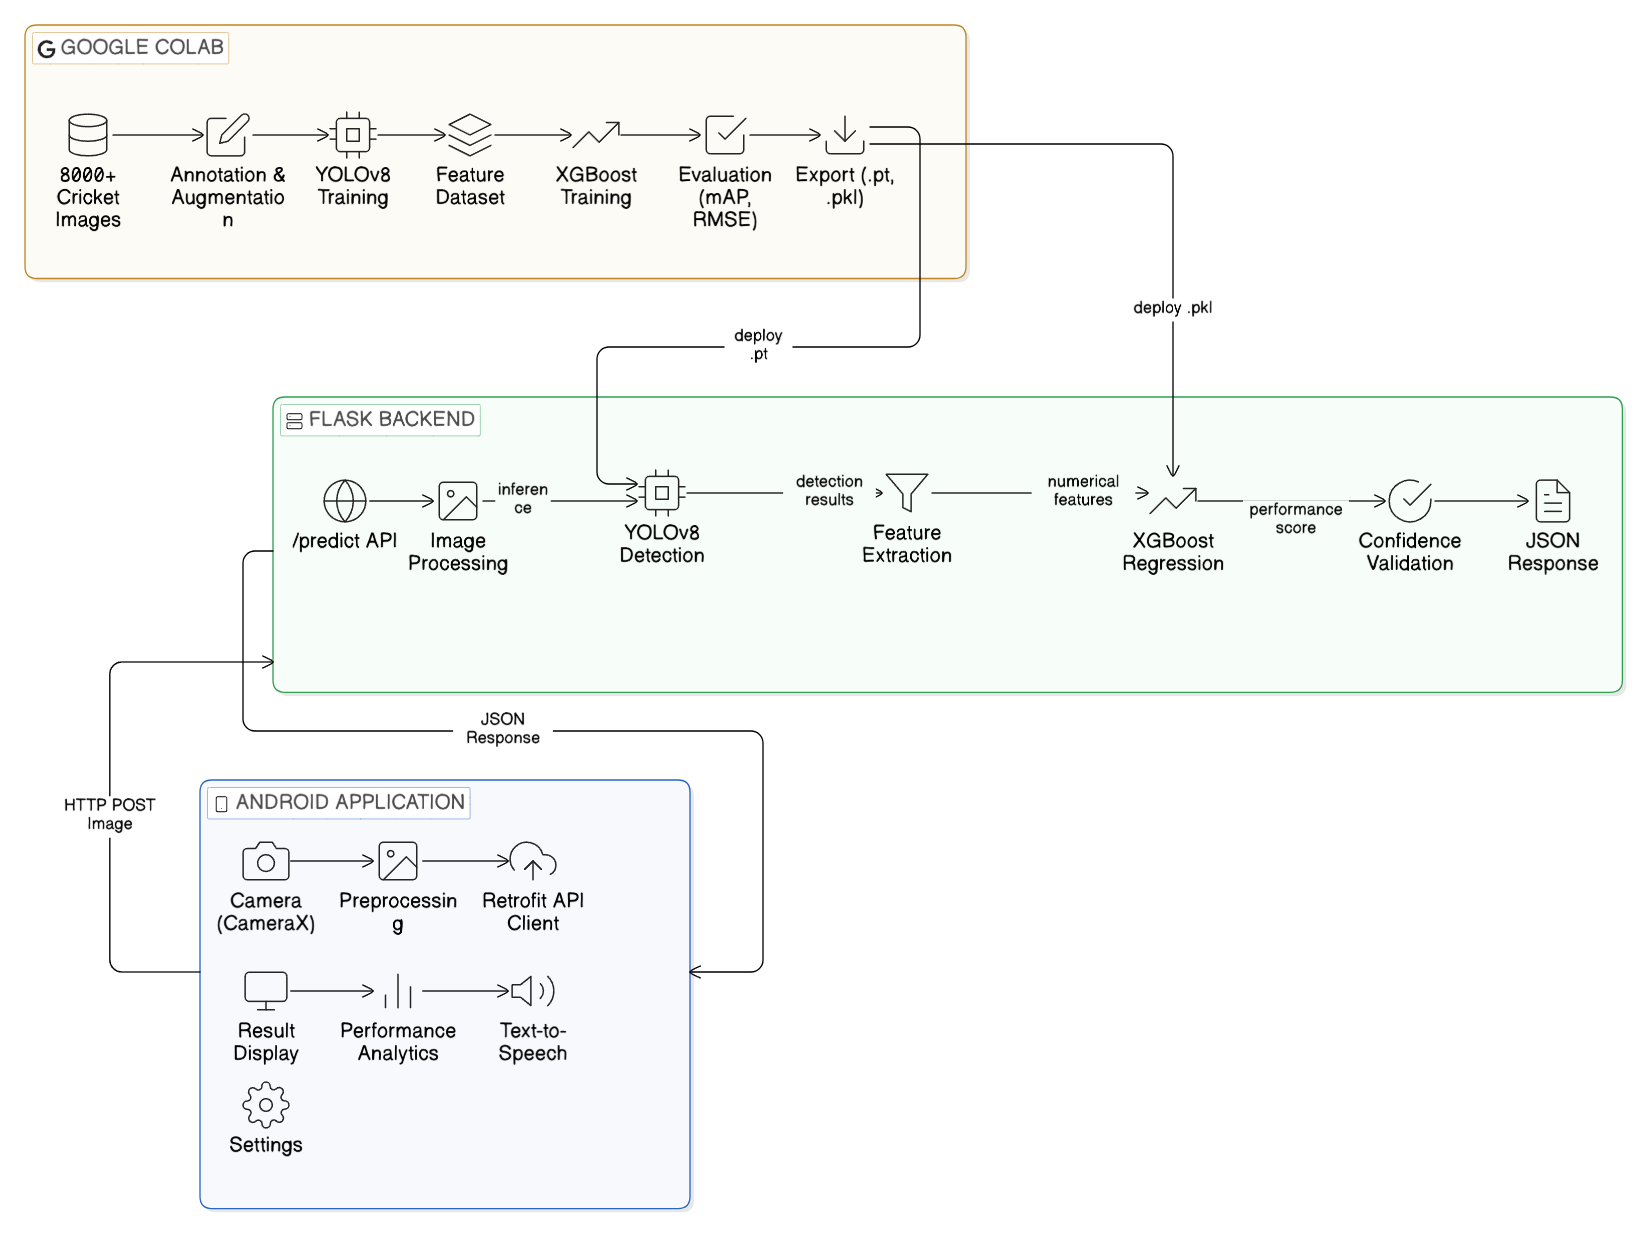
\includegraphics[width=1.2\linewidth]{Figures/Chapter-5figs/architecture_diagram}
	\caption{Architecture Diagram}
	\label{fig:architecture}
\end{figure}

\textit{Description:-}

The Fig.5.1. illustrates the architecture of the AI-Powered Cricket Shot Classification System consists of three main layers: the Training Environment, Client Layer, and Server Layer. In the training phase, a YOLOv8 model is developed using Google Colab with over 8000 cricket batting images, applying data augmentation, training, and evaluation before exporting the trained model as an `.h5` file for deployment. The Client Layer includes an Android application that captures batting images using CameraX, preprocesses them, and sends them to the Flask backend via an HTTP POST request. The Server Layer handles authentication, image preprocessing, and model inference using a YOLOv8 model to classify the shot as straight drive, pull shot, cut shot, or sweep. Based on a confidence threshold, the system either returns a valid prediction or marks it as unknown. The final result is sent back as a JSON response, displayed in the app, and announced through a Text-to-Speech module, enabling real-time and user-friendly shot analysis.

\section{Flow Chart} \label{S5.2}

\textit{Description:-}

The Fig. 5.2. illustrates the working process of the proposed cricket shot classification system. The process begins when the user opens the Android application and captures a batting image using the device camera. The captured image undergoes initial preprocessing on the mobile device, such as resizing and normalization, to ensure it meets the required input format. The preprocessed image is then transmitted to the backend server for further analysis. Upon receiving the image, the server performs additional preprocessing steps if necessary and forwards the image to the YOLOv8 model for shot detection and classification. The YOLOv8 model extracts relevant features, identifies the batting posture, and predicts the corresponding shot along with a confidence score. The system then evaluates whether the predicted confidence score meets a predefined threshold. If the confidence is greater than or equal to the threshold, the shot is marked as a valid prediction; otherwise, it is classified as an unknown shot to avoid incorrect outputs. After classification, a structured JSON response containing the predicted shot label and confidence value is generated and sent back to the Android application. The application receives the response, displays the predicted shot on the screen, and provides voice feedback to enhance user interaction.

\begin{figure}[H]
	\centering
	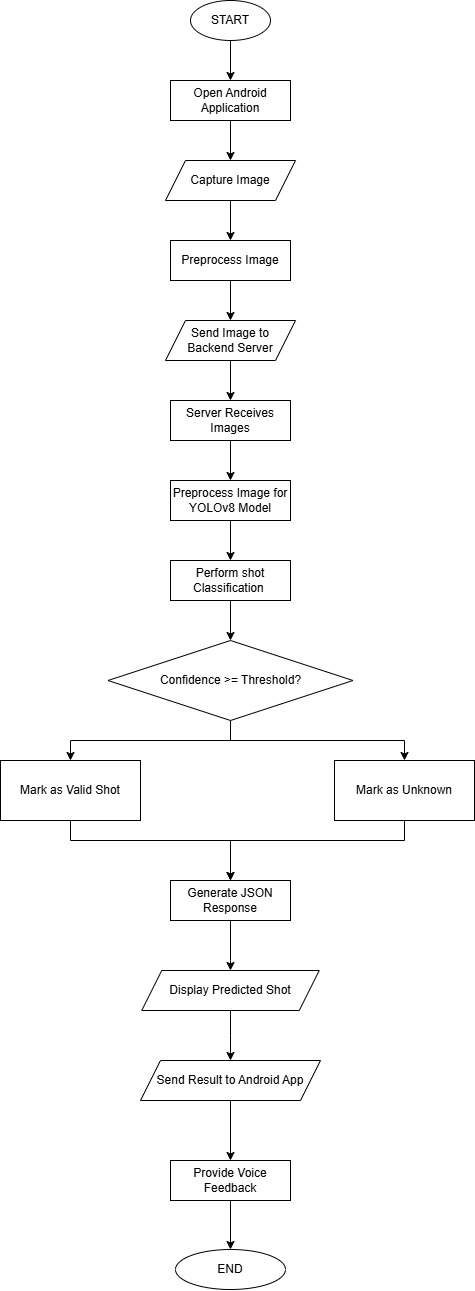
\includegraphics[width=0.55\linewidth]{Figures/Chapter-5figs/flow_chart}
	\caption{Flow Chart}
	\label{fig:flowchart}
\end{figure}
 
\section{Use Case Diagram} \label{S5.3}
\begin{figure}[H]
	\centering
	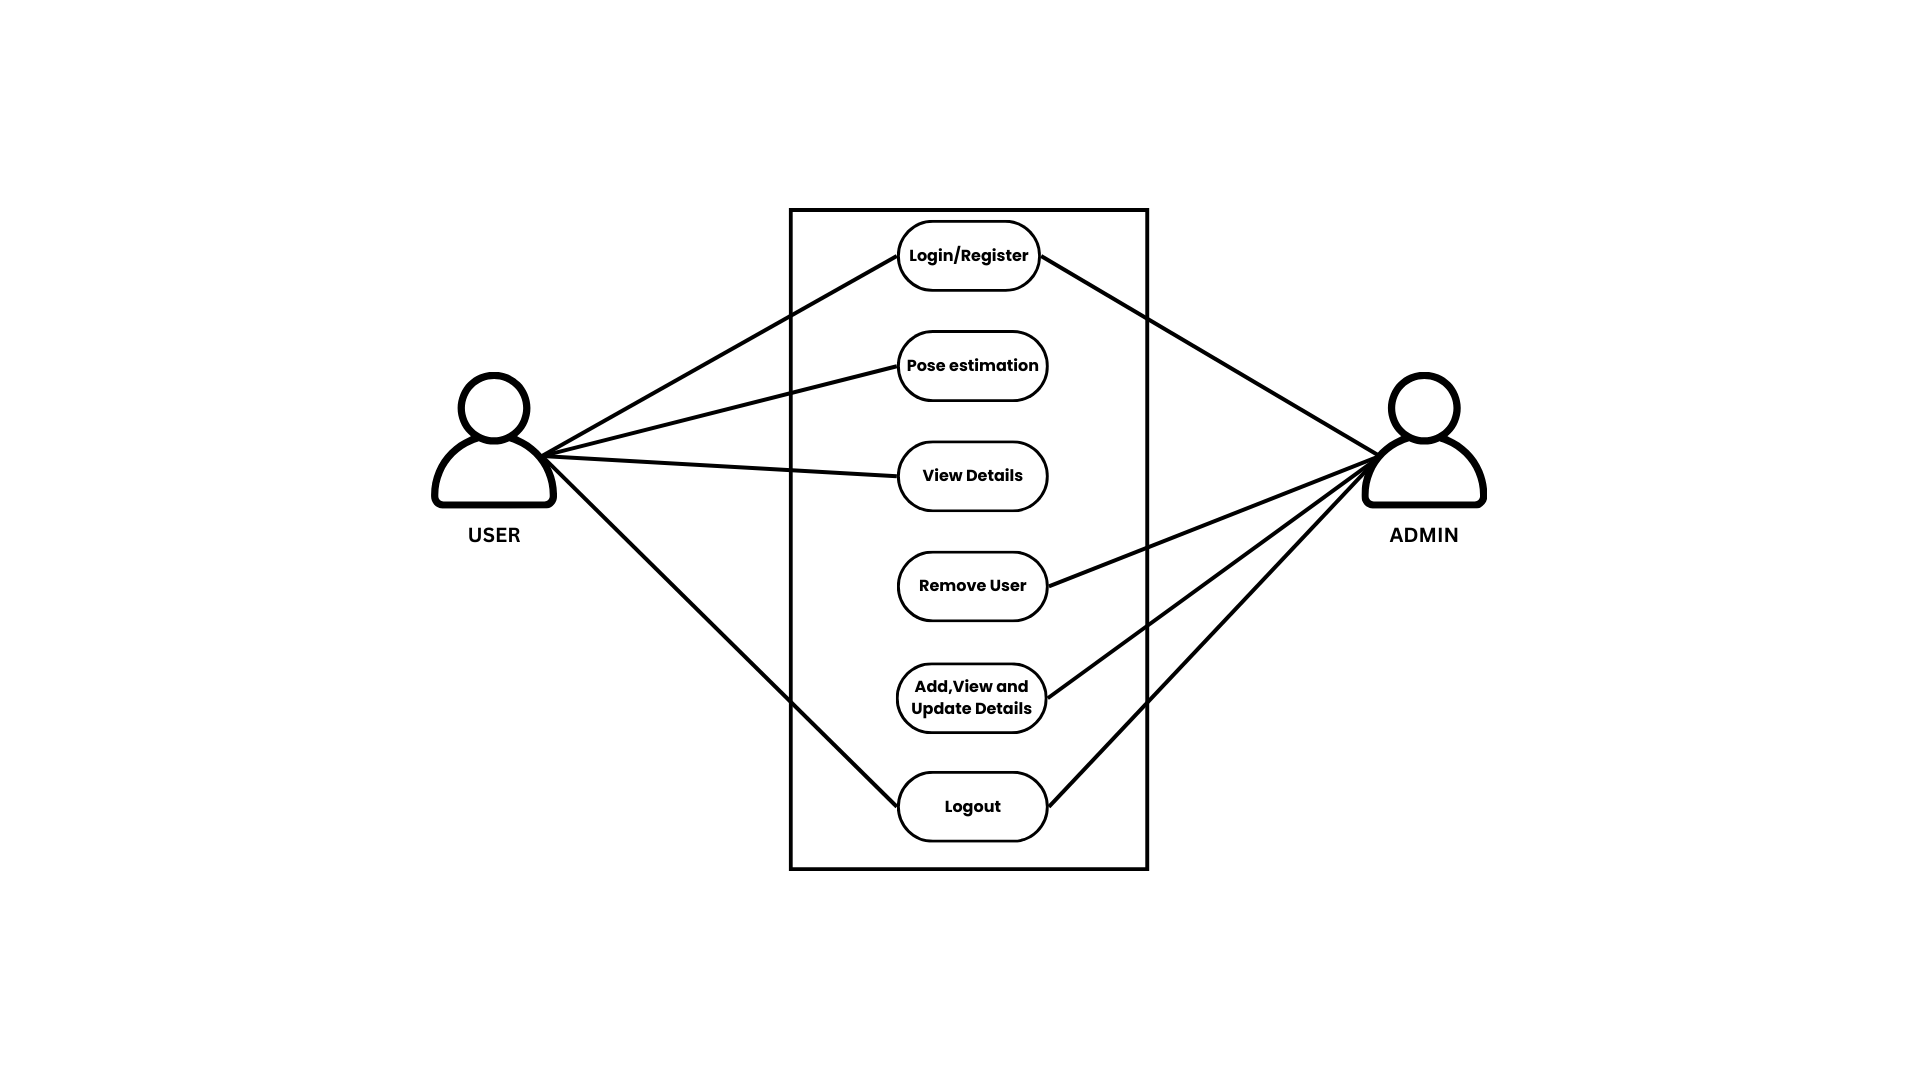
\includegraphics[width=1.05\linewidth]{Figures/Chapter-5figs/use_case_diagram}
	\caption{Use Case Diagram}
	\label{fig:usecase}
\end{figure}

\textit{Description:-}

Fig. 5.3 represents the Use Case Diagram of the proposed cricket shot analysis system, illustrating the interaction between two primary actors: the User and the Admin. The diagram highlights the functional requirements of the system within a defined system boundary. The User actor is associated with fundamental operations such as Login/Register, which enables secure authentication and account creation; Pose Estimation, which allows the user to upload or capture images for pose detection and shot analysis; and View Details, through which the user can access prediction results, performance insights, or related information.
The Admin actor possesses higher-level privileges to manage and control the system effectively. In addition to Login/Register functionality, the Admin can Remove User accounts to maintain system integrity and handle unauthorized access. The Admin is also responsible for Add, View, and Update Details, which may include managing shot categories, updating model-related information, maintaining user records, and overseeing stored data. 

\section{Activity Diagram} \label{S5.4}

\begin{figure}[H]
	\centering
	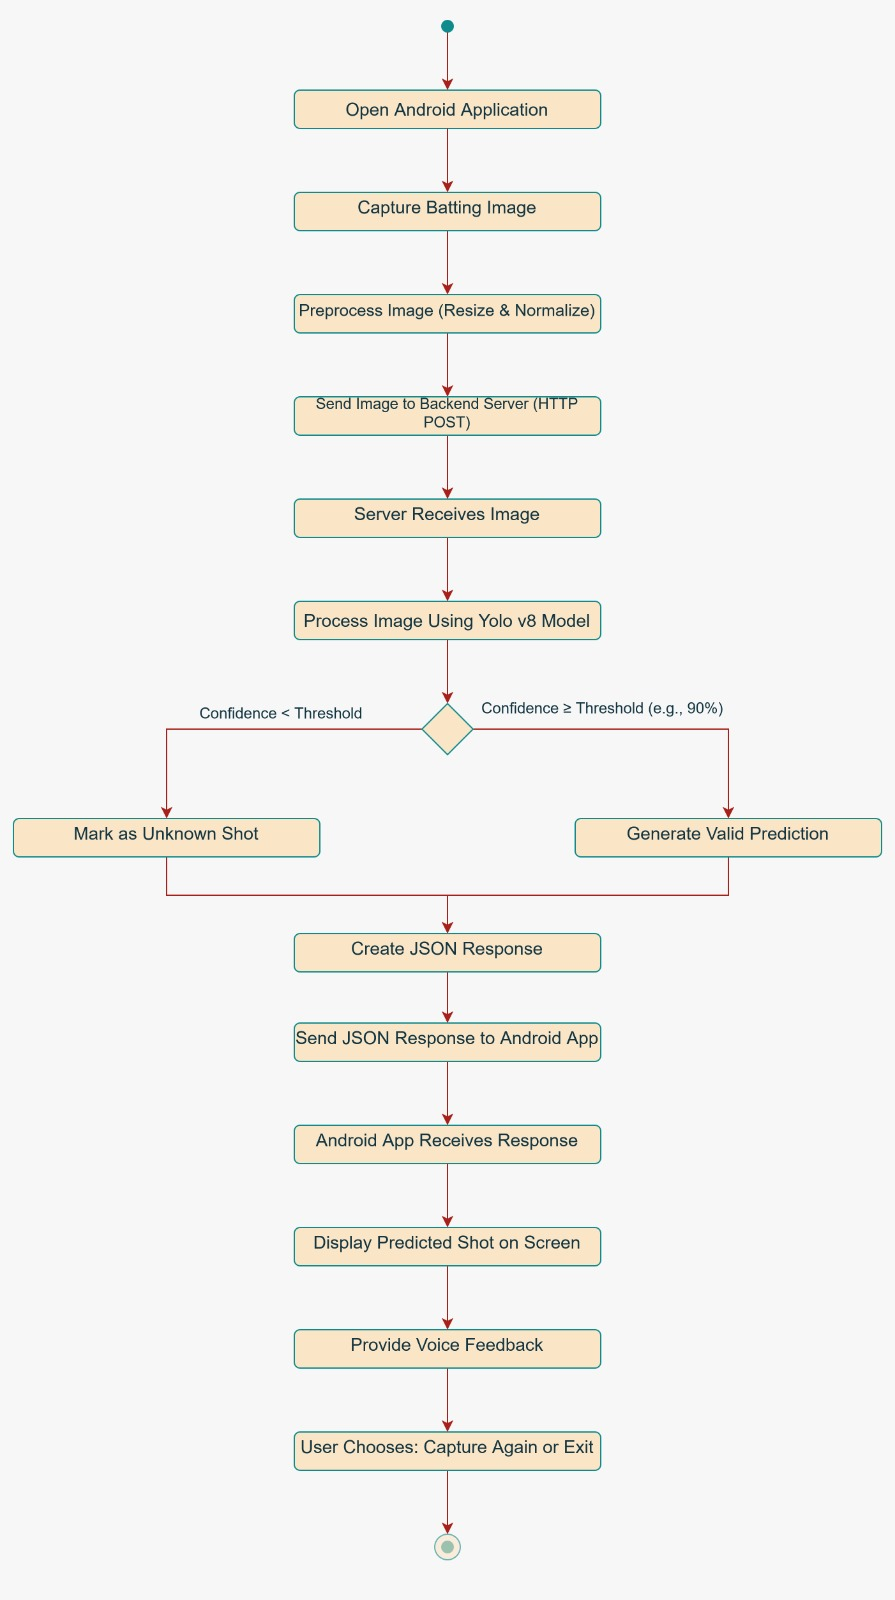
\includegraphics[width=0.8\linewidth]{Figures/Chapter-5figs/activity_diagram}
	\caption{Activity Diagram}
	\label{fig:activity}
\end{figure}

\textit{Description:-}

The Fig.5.4. is the activity diagram which illustrates the operational workflow of the Android-based cricket shot classification system. The process starts when the user opens the Android application and captures a batting image, which is then preprocessed by resizing and normalizing before being sent to the backend server via an HTTP POST request. The server receives the image and processes it using the YOLOv8 model to perform shot classification. A decision node evaluates whether the prediction confidence meets a predefined threshold (which is 90\%); if the confidence is below the threshold, the shot is marked as unknown, otherwise a valid prediction is generated. The system then creates a JSON response and sends it back to the Android application, where the result is received, displayed on the screen, and supported with voice feedback. Finally, the user decides whether to capture another image or exit the application, completing the activity flow.

\section{Sequence Diagram} \label{S5.5}

\textit{Description:-}

The Fig.5.5. illustrates the end-to-end workflow of the AI-Powered Cricket Shot Classification System. The process begins when the user opens the Android application and captures a batting image, which is then preprocessed (resized and normalized) within the app before being sent to the Flask backend server via an HTTP POST request. The server further preprocesses the image and forwards it to the YOLOv8 model for shot classification. The model returns a predicted label straight drive, pull shot, cut shot, or sweep along with a probability score. The server performs a confidence threshold check to determine whether the prediction is valid or should be marked as unknown. It then sends a JSON response containing the prediction and encoded image back to the Android application. Finally, the app displays the predicted result to the user and sends the label to the Text-to-Speech module, which announces the detected cricket shot.

\begin{figure}[H]
	\centering
	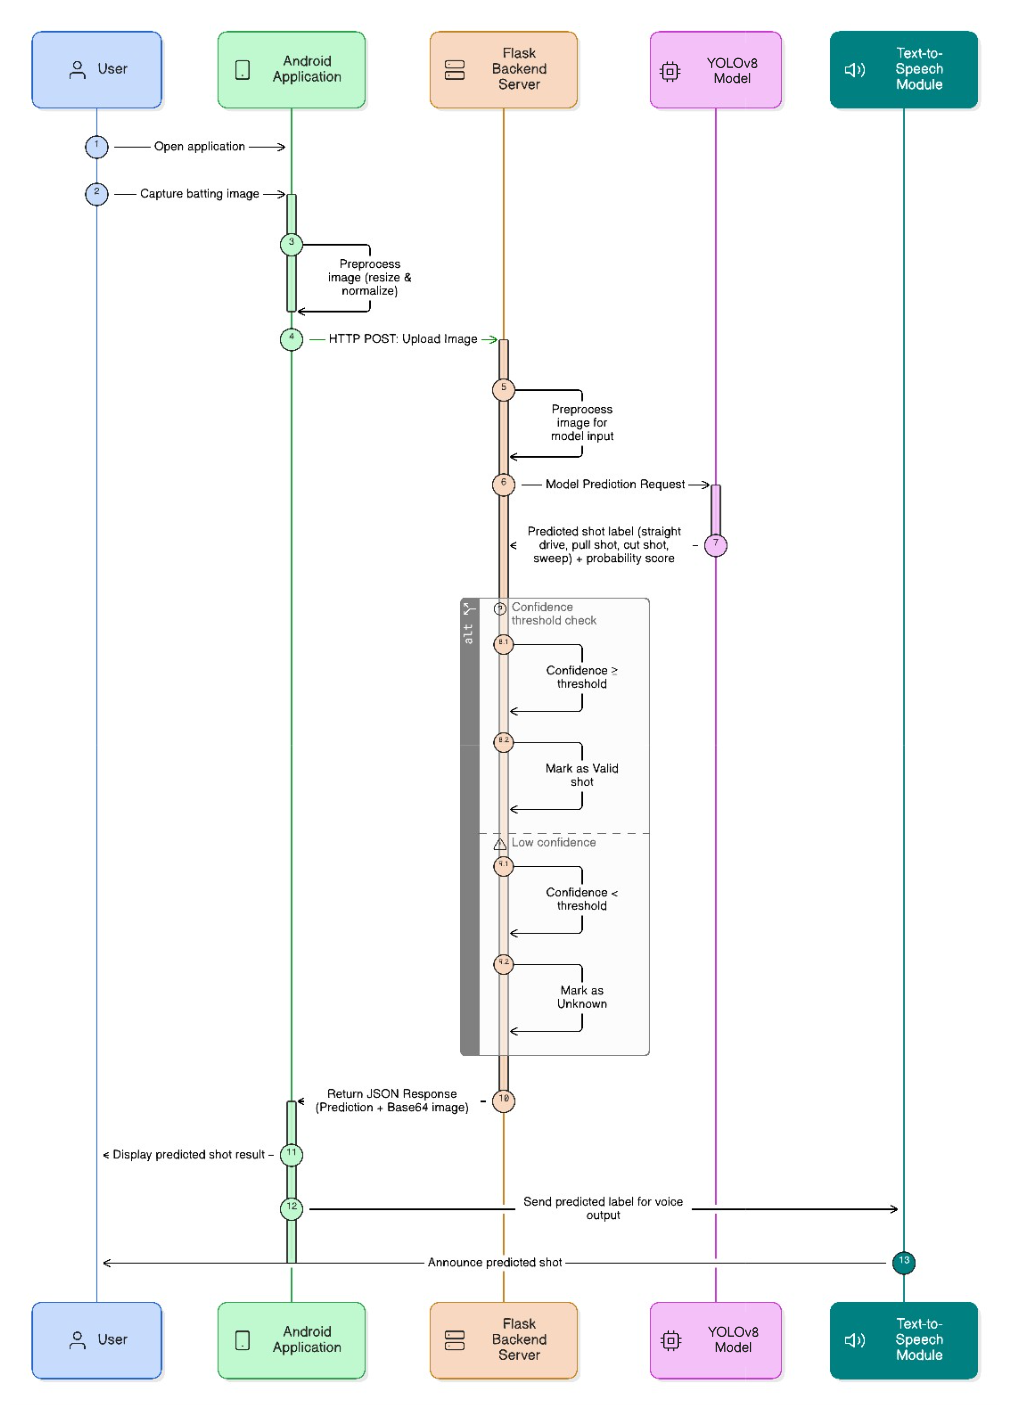
\includegraphics[width=1.05\linewidth]{Figures/Chapter-5figs/sequence_diagram}
	\caption{Sequence Diagram}
	\label{fig:sequence}
\end{figure}

\section{Collaboration Diagram} \label{S5.6}
\begin{figure}[H]
	\centering
	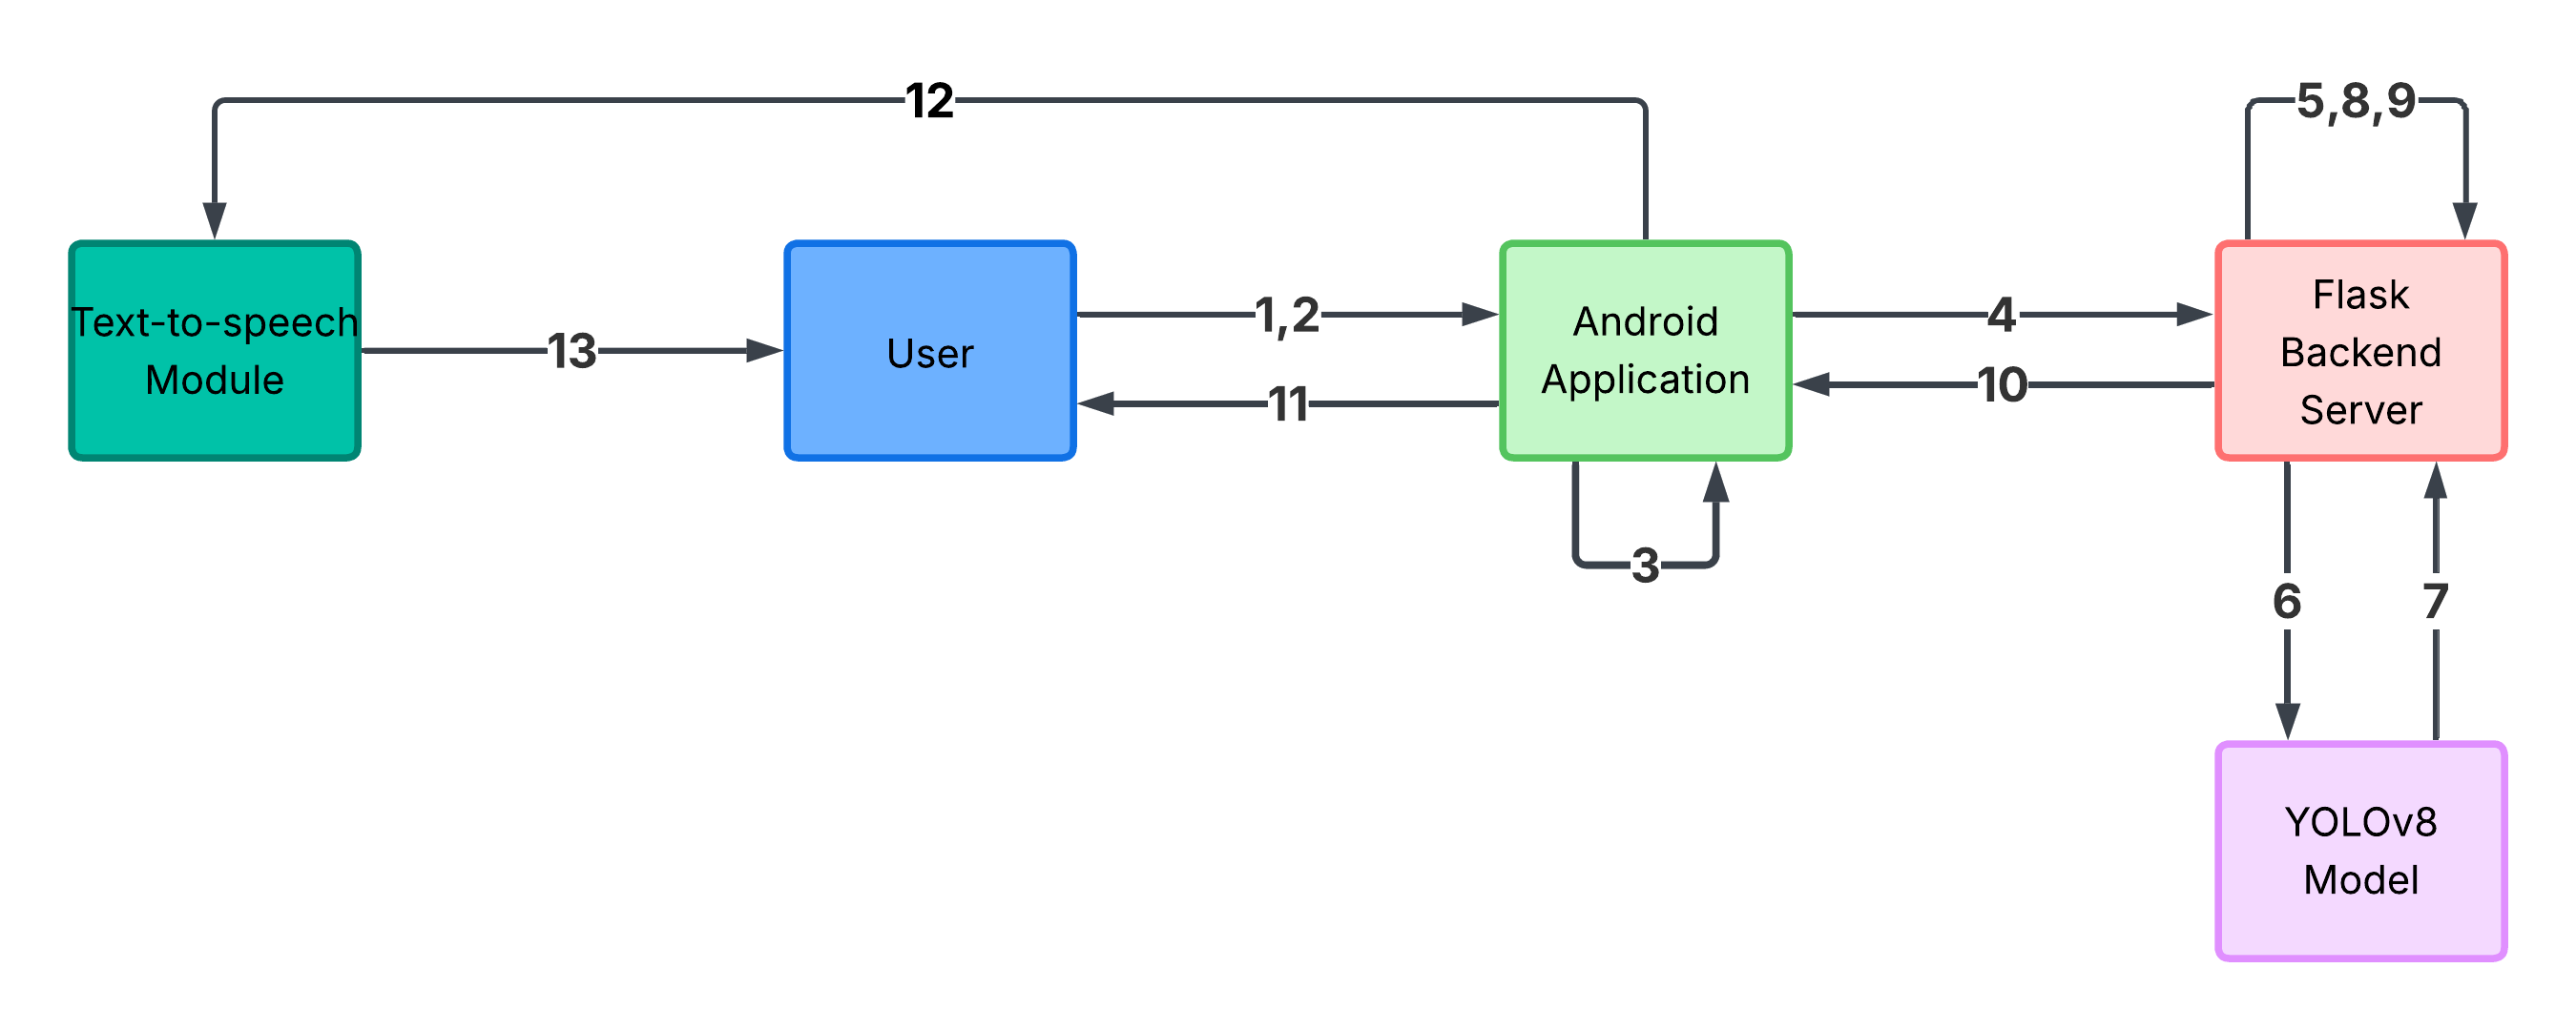
\includegraphics[width=0.95\linewidth]{Figures/Chapter-5figs/collaboration_diagram}
	\caption{Collaboration Diagram}
	\label{fig:collab}
\end{figure}

\textit{Description:-}

The Fig.5.6. illustrates the interaction between the User, Android Application, Flask Backend Server, YOLOv8 Model, and Text-to-Speech Module in the AI-Powered Cricket Shot Classification System. The process begins with the user opening the application and capturing a batting image through the Android app. The app preprocesses the image and sends it to the Flask backend server via an HTTP request. The server forwards the processed image to the YOLOv8 model for classification, which predicts the shot type straight drive, pull shot, cut shot, or sweep and returns a probability score. The server evaluates the confidence level, prepares a JSON response, and sends the prediction back to the Android application. The app then displays the result to the user and forwards the predicted label to the Text-to-Speech module, which announces the detected cricket shot, completing the interaction flow.

%%%%%%%%%%%%%%%%%%%%%%%%%%%%%%%%%%%%%%%%%%%%%%%%%%%%%%%%%%%%%%%%%%%%%%%%%%%%%%%%%%%%%%%%%%%%%%%%%%%%%%%%%%%%%%%%%%%%%%%%%%%%%%%%%%%%%%%%
